\documentclass[a4paper,12pt]{article}
\usepackage[english,ukrainian,russian]{babel}
\linespread{1}
\usepackage{ucs}
\usepackage[utf8]{inputenc}
\usepackage[T2A]{fontenc}
\usepackage[paper=portrait,pagesize]{typearea}
\usepackage{amsmath}
\usepackage{bigints}
\usepackage{amsfonts}
\usepackage{graphicx}
\usepackage{amssymb}
\usepackage{cancel}
\usepackage{gensymb}
\usepackage{multirow}
\usepackage{rotate} 
\usepackage{pdflscape}
\usepackage{bigstrut}
\usepackage[pageanchor]{hyperref}
\usepackage{chngpage}
\newcommand{\dx}{\textbf{d}x}
\newcommand{\dt}{\textbf{d}t}
\newcommand{\du}{\textbf{d}u}
\newcommand{\dv}{\textbf{d}v}
\newcommand{\dy}{\textbf{d}y}
\newcommand{\ds}{\textbf{d}s}
\newcommand{\dz}{\textbf{d}z}
\newcommand{\arch}{\textrm{arcch}}
\newcommand{\arsh}{\textrm{arcsh}}
\newcommand{\dint}{\displaystyle\int}
\newcommand\tab[1][1cm]{\hspace*{#1}}
\newcommand{\dsum}{\displaystyle\sum}
\newcommand{\RomanNumeralCaps}[1]{\MakeUppercase{\romannumeral #1}}
\usepackage[left=20mm, top=20mm, right=15mm, bottom=15mm, nohead, nofoot]{geometry}
\usepackage{verbatim}

\usepackage{listings}
\usepackage{xcolor}

\definecolor{codegreen}{rgb}{0,0.6,0}
\definecolor{codegray}{rgb}{0.5,0.5,0.5}
\definecolor{codepurple}{rgb}{0.58,0,0.82}
\definecolor{backcolour}{rgb}{0.95,0.95,0.92}

\lstdefinestyle{mystyle}{
	backgroundcolor=\color{backcolour},   
	commentstyle=\color{codegreen},
	keywordstyle=\color{blue},
	numberstyle=\tiny\color{codegray},
	stringstyle=\color{red},
	basicstyle=\ttfamily\footnotesize,
	breakatwhitespace=false,         
	breaklines=true,                 
	captionpos=b,                    
	keepspaces=true,                 
	numbers=none,                    
	numbersep=5pt,                  
	showspaces=false,                
	showstringspaces=false,
	showtabs=false,                  
	tabsize=4,
	frame=shadowbox
}

\lstset{style=mystyle}

\begin{document}
\begin{center}
    \hfill \break
    \large{\textbf{НАЦIОНАЛЬНИЙ ТЕХНIЧНИЙ УНIВЕРСИТЕТ УКРАЇНИ\\
            «КИЇВСЬКИЙ ПОЛIТЕХНIЧНИЙ IНСТИТУТ»\\
            НАВЧАЛЬНО-НАУКОВИЙ ФІЗИКО-ТЕХНІЧНИЙ ІНСТИТУТ}}\\
    \hfill \break \hfill \break \hfill\break \hfill \break \hfill \break \hfill \break \hfill \break
    \hfill \break \hfill \break
    \large{КУРСОВА РОБОТА}
    \begin{center}
        \normalsize{\textbf{з дисципліни «Спеціальні розділи програмування» \\
        На тему: «Знайомство з можливостями Anaconda/IPython Notebook. \\
        Аналіз та візуалізація даних датасету» \\}}
    \end{center}
\end{center}
\hfill \break \hfill \break \hfill \break \hfill \break \hfill \break \hfill \break \hfill \break
\hfill \break \hfill \break \hfill \break \hfill \break \hfill \break \hfill \break 
\begin{flushright}
    \large{ \hspace{35pt} Виконав:\\
        студент групи ФI-12\\
        Завалій Олександр} 
\end{flushright}
\hfill \break \hfill \break \hfill \break \hfill \break \hfill \break \hfill \break \hfill \break
\hfill \break \hfill \break 
\begin{center} \textbf{Київ-2022} \end{center}
\thispagestyle{empty}



\newpage
    \renewcommand*\contentsname{Contents}
    \tableofcontents


\newpage
    \section {Частина}
    \subsection {Знайомство з можливостями Anaconda/IPython Notebook}
    \hrulefill \\
    Для того, щоб почати працювати з Anaconda потрібно її встановити:
    \begin{enumerate}
        \item Перейти на офіційний сайт \href{https://www.anaconda.com/products/distribution}{\underline{Anaconda Distribution}} 
        та натиснути кнопку "Download". Також можна безкоштовно спробувати Anaconda в вашому браузері після реєстрації.
        \begin{figure}[h!]
            \begin{center}
                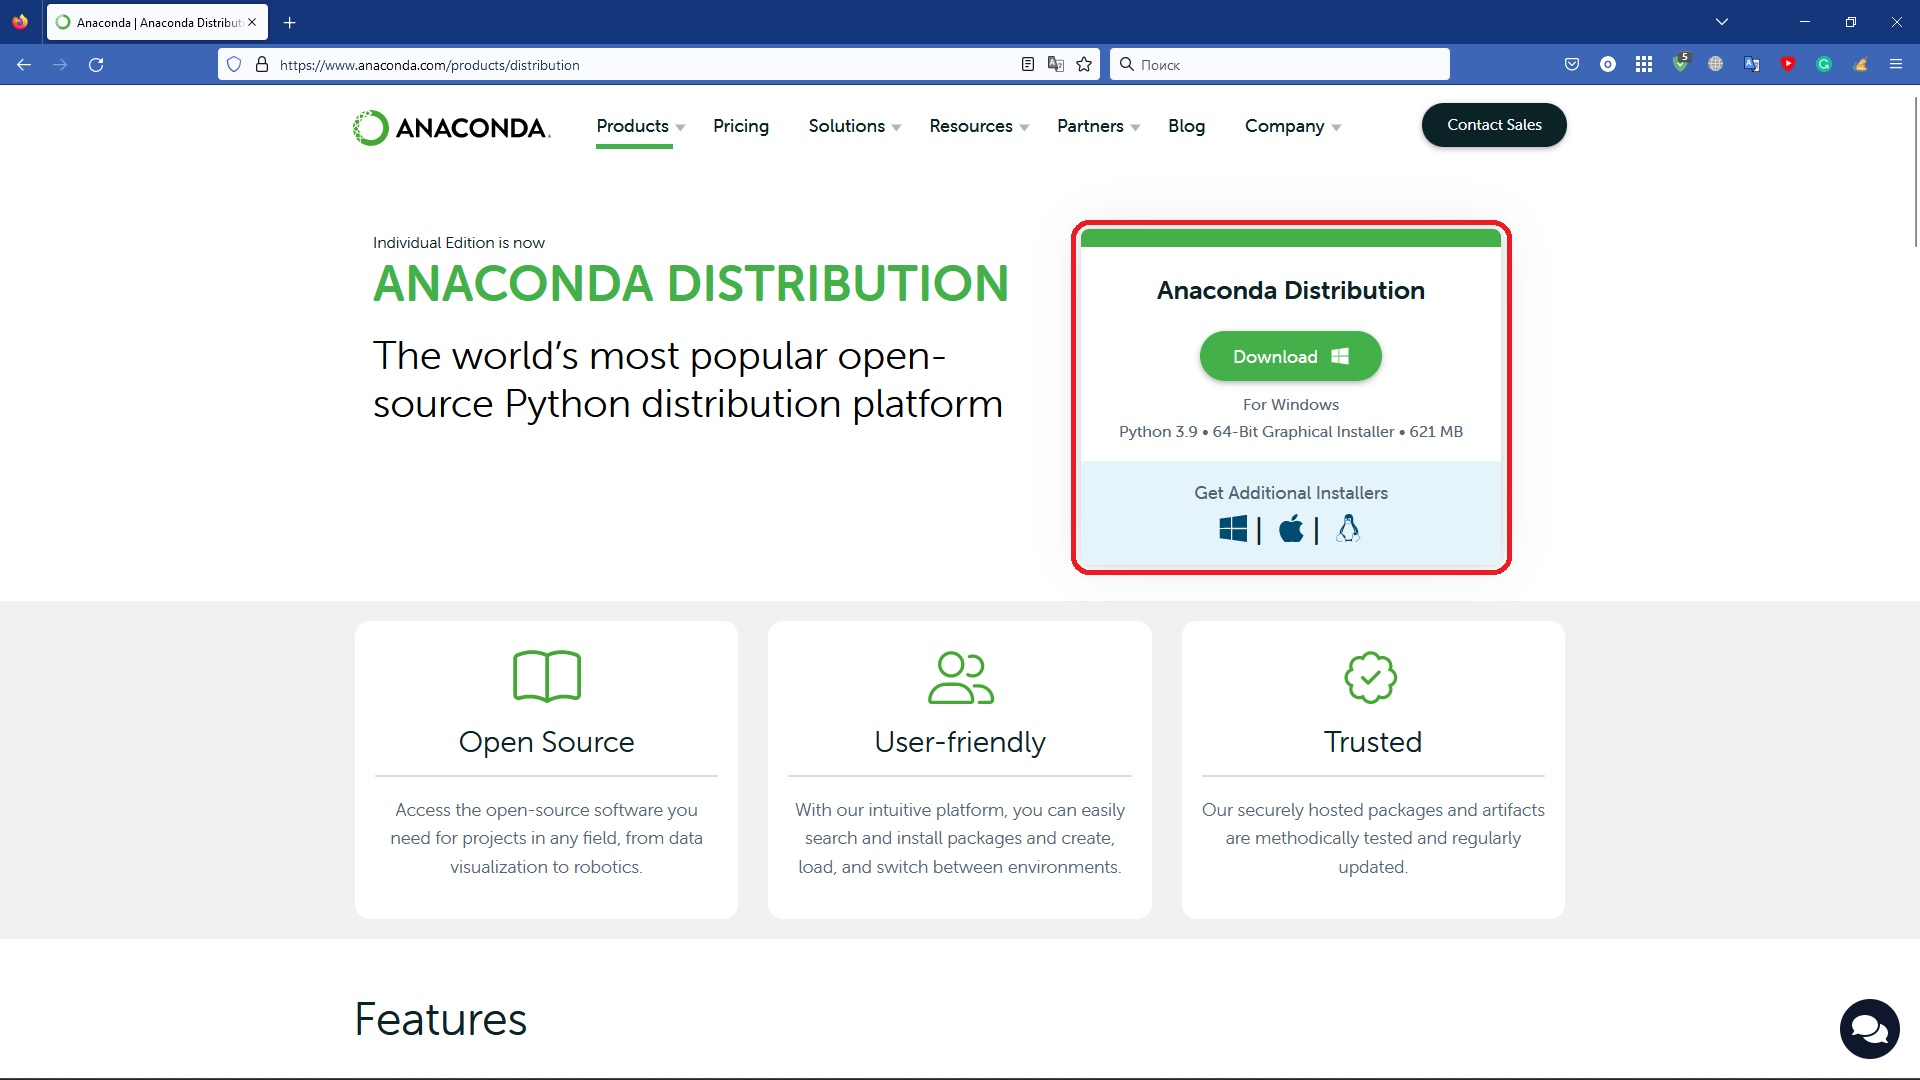
\includegraphics[scale=0.35]{Prt sc/Figure_1.jpg}
            \end{center}
        \end{figure}
        \item Після завантаження встановлюємо застосунок. Отримаємо таке повідомлення.
        \begin{figure}[h!]
            \begin{center}
                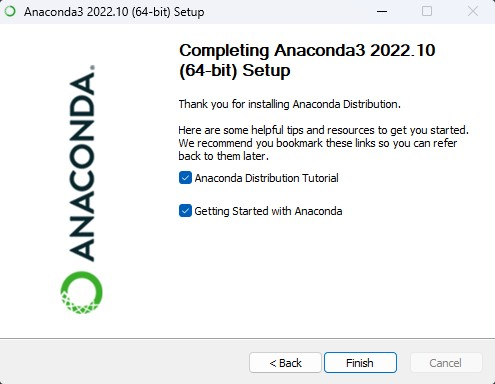
\includegraphics[scale=0.8]{Prt sc/Figure_2.jpg}
            \end{center}
        \end{figure}
\newpage
        \item Далі відкриваємо застосунок Anaconda Navigator і обираємо Jupyter Notebook. Або одразу відкрити Jupyter Notebook. Він знаходиться в папці, 
        куди була встановлена Anaconda.
        \begin{figure}[h!]
            \begin{center}
                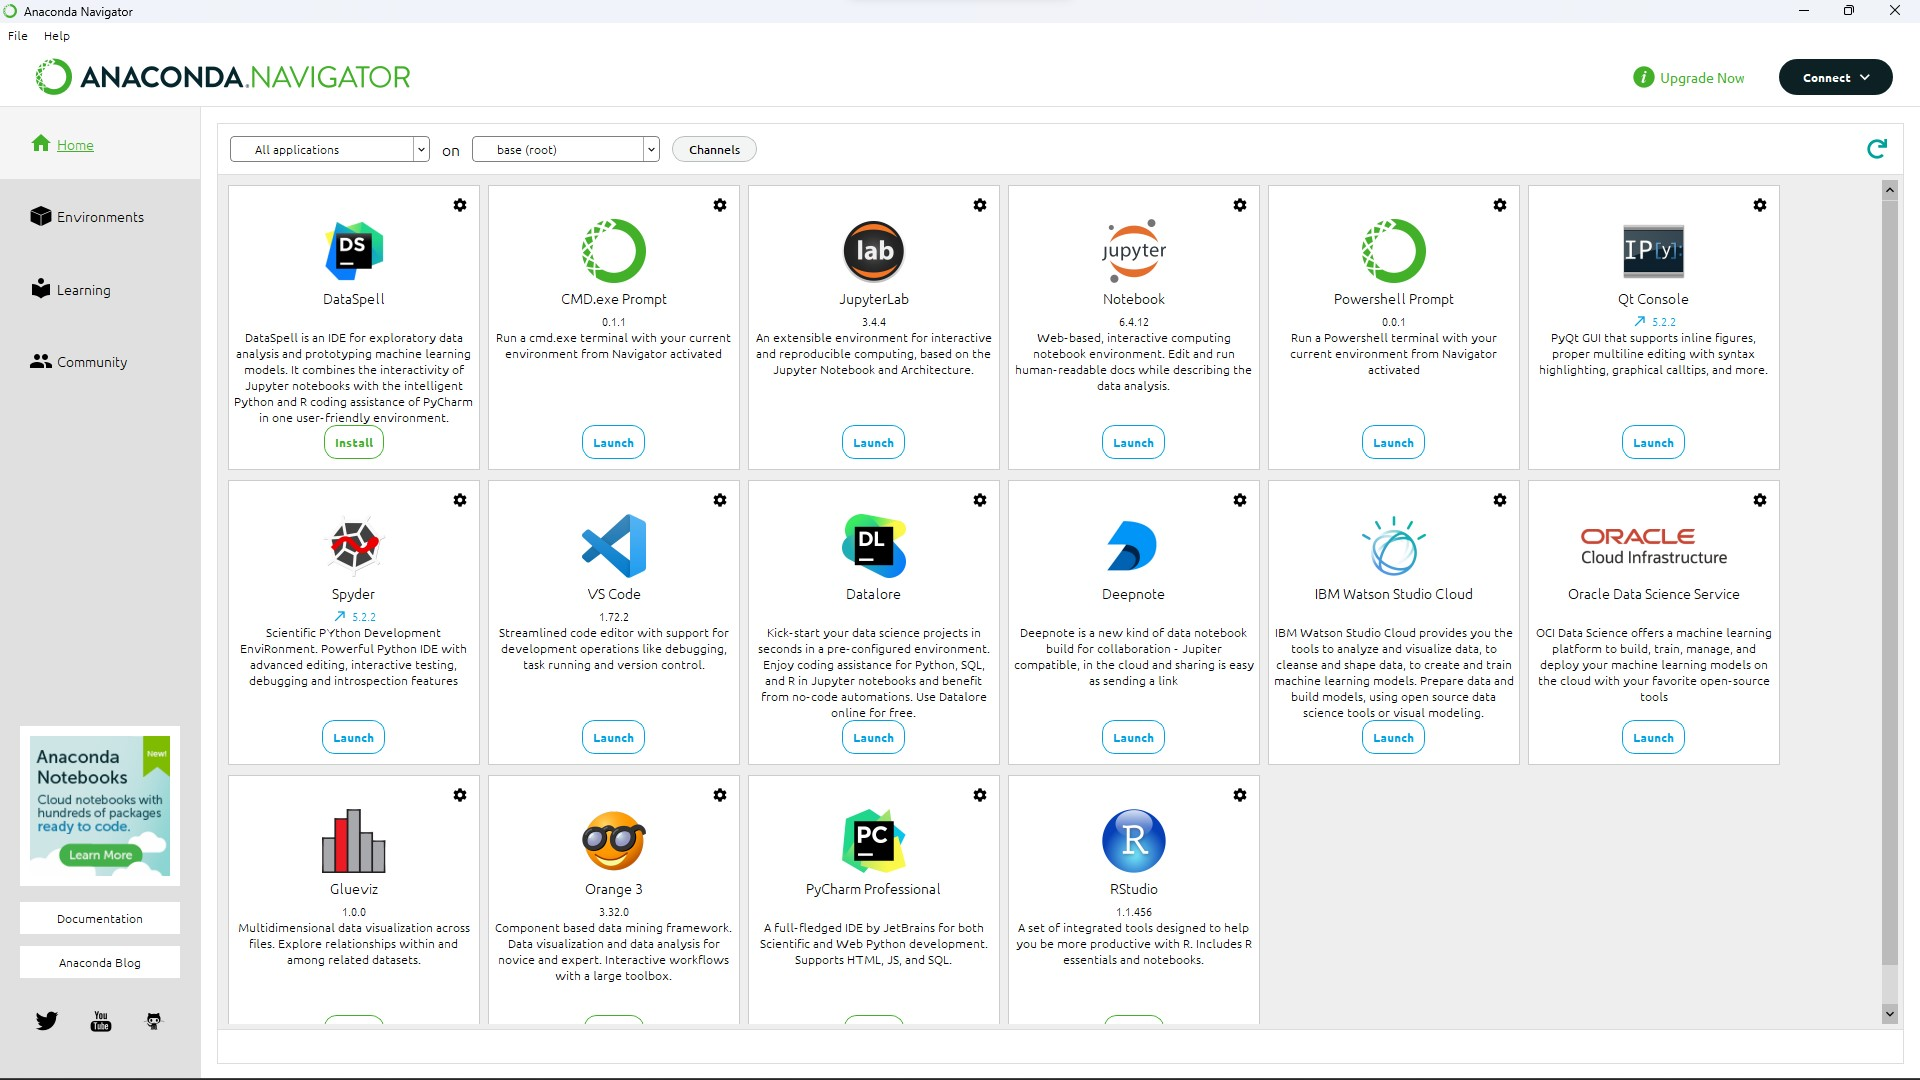
\includegraphics[scale=0.35]{Prt sc/Figure_3.jpg}
            \end{center}
        \end{figure}
        \item Ось так виглядає Jupyter Notebook.
        \begin{figure}[h!]
            \begin{center}
                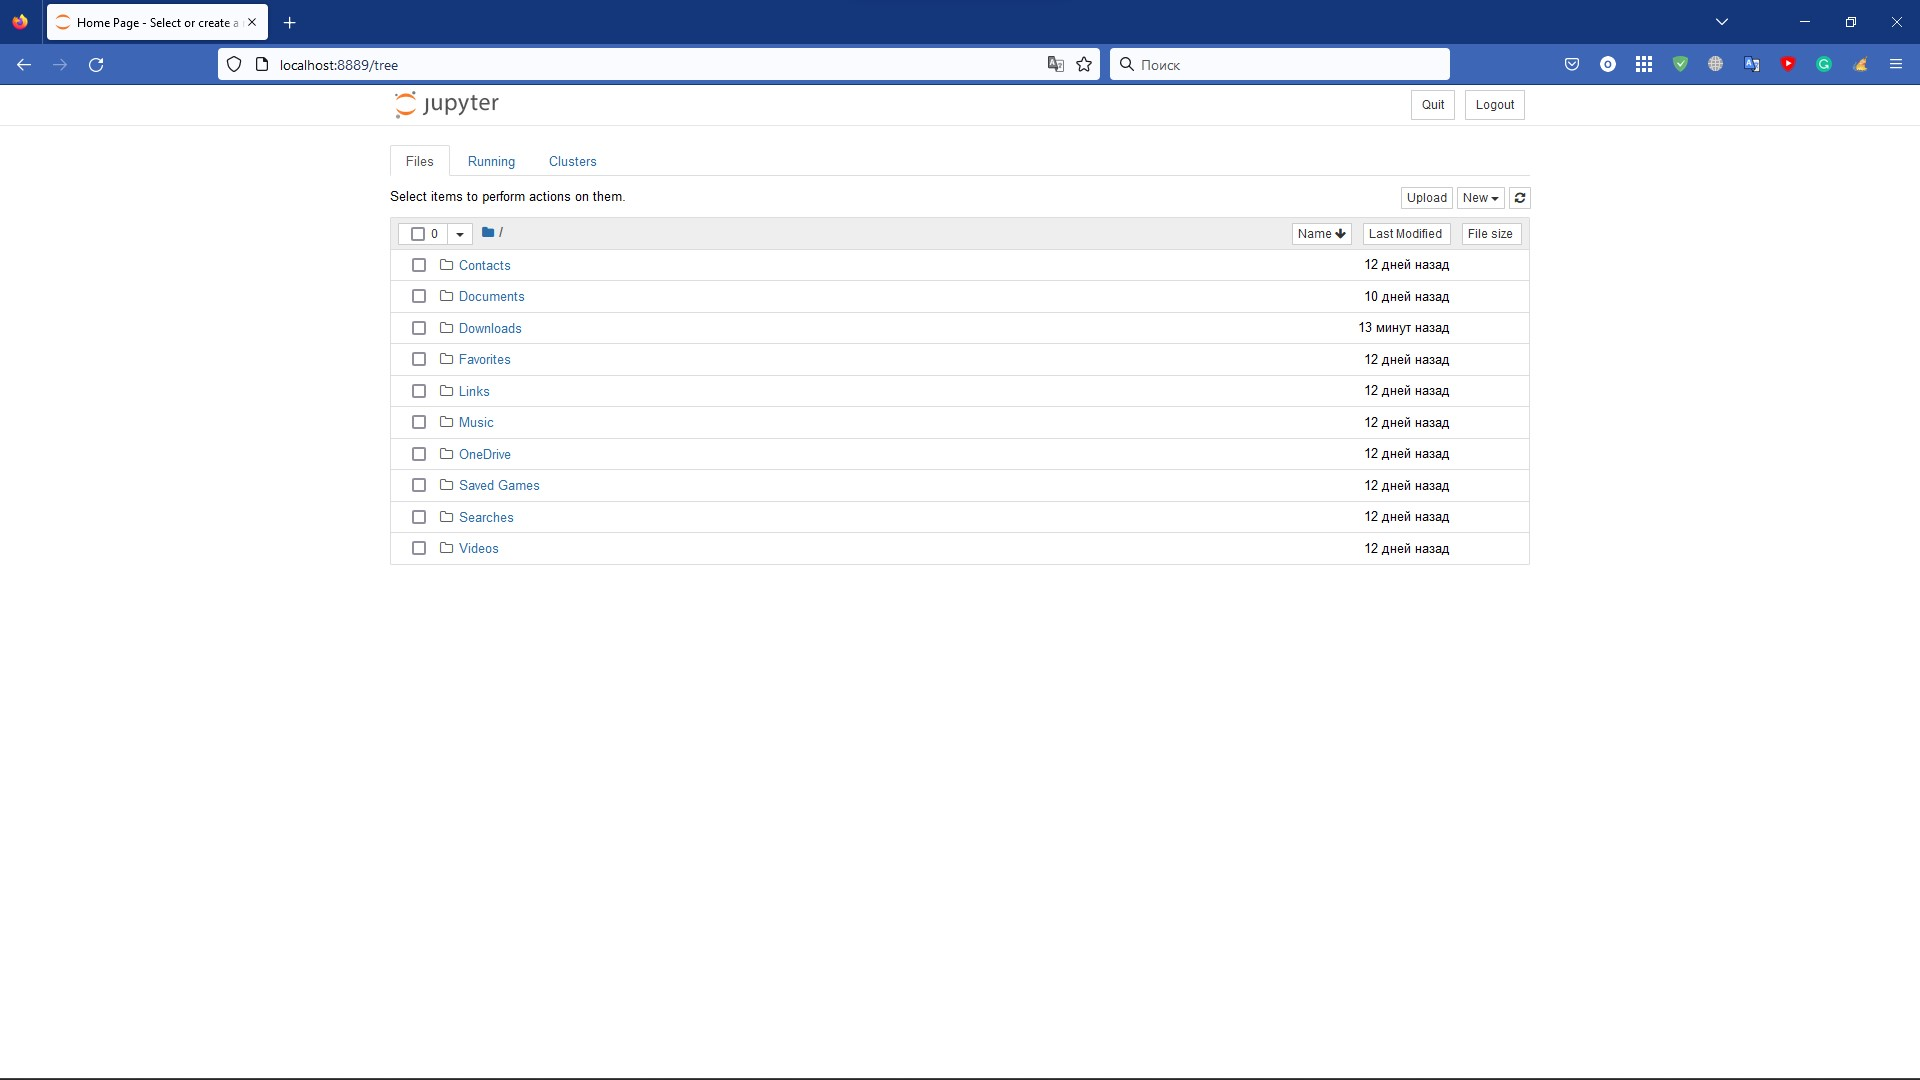
\includegraphics[scale=0.35]{Prt sc/Figure_4.jpg}
            \end{center}
        \end{figure}
    \end{enumerate}
\newpage
    \subsection{IPython Notebook та Visual Studio Code.}
    \hrulefill \\
    Надалі я буду працювати з IPython Notebook у редакторі вихідного коду Visual Studio Code. Нижче наведені переваги використання VC Code.
    \begin{enumerate}
        \item Редактор VC Code підтримує декілька мов програмування, у тому числі: JavaScript, C++, PHP, Python, Java, Objective-C, PowerShell,
        Visual Basic, Markdown, JSON, HTML, CSS... Тому дуже просто писати код в IPython Notebook в одній вкладці, та паралельно редагувати Latex документ наприклад.
        \item Data viewer. Провідник змінних Jupyter Variables показує додаткову корисну інформацію про розмір і тип кожної змінної. 
        Також є можливість переглядати DataFrame або Series на окремій вкладці, щоб не завантажувати файли на інші платформи для перегляду.
        \item Code formatting. Використовується формат коду, такий як \href{https://github.com/google/yapf}{\underline{yapf}} або 
        \href{https://github.com/psf/black}{\underline{black}}, для форматування більш складного коду pandas. 
        VS Code застосує вибраний формататор, щоб очистити ваш вкладений код.
        \item Split editors. Дуже просто писати код в IPython Notebook в одній вкладці, та паралельно редагувати Latex документ в іншій вкладці.
        \item Git integration. VS Code легко інтегрується з git.
        \item Change kernels. Якщо ви використовуєте conda або віртуальне середовище, дуже корисно мати можливість швидко змінити середовище.
        \item Supports WSL. VS Code добре інтегрується з WSL, тому ви можете розробляти на Windows або Linux.
        \item Plugins. 
    \end{enumerate}
\newpage
    \subsection {Почнемо знайомство з Jupyter Notebook у Visual Studio Code.}
    \hrulefill \\
    Для того, щоб працювати з Jupyter Notebook у Visual Studio Code потрібно:
    \begin{enumerate}
        \item Перейти на офіційний сайт \href{https://code.visualstudio.com/}{\underline{Visual Studio Code}} і завантажити редактор коду.
        \item Натиснути комбінацію клавіш "Ctrl+Shift+X", відкриється  розділ "Extensions", тут потрібно завантажити Python. 
        \item Створюємо або відкриваємо папку у VS Code explorer.
        \item Натискаємо "File--New File--Jupyter Notebook"
        \begin{figure}[h!]
            \begin{center}
                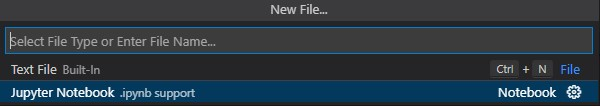
\includegraphics[scale=0.9]{Prt sc/Figure_5.jpg}
            \end{center}
        \end{figure}
        \item Зберігаємо файл у папці.
    \end{enumerate}
    \hrulefill
    \begin{center}
        \subsubsection{Довідка по плагіну "Python".}
    \end{center}
    \hrulefill 

    Цей плагін офіційно був створений та підтримується компанією Microsoft. Розширення включає такі функції, як 
    IntelliSense (Pylance), linting, debugging, code navigation, code formatting, refactoring, variable explorer, test explorer, тощо. 

    Тобто Python автоматично встановить розширення \href{https://marketplace.visualstudio.com/items?itemName=ms-python.vscode-pylance}{\underline{Pylance}}
    та \href{https://marketplace.visualstudio.com/items?itemName=ms-toolsai.jupyter}{\underline{Jupyter}}, щоб забезпечити вам найкращий досвід роботи з файлами Python 
    і блокнотами Jupyter. 
    \begin{figure}[h!]
        \begin{center}
            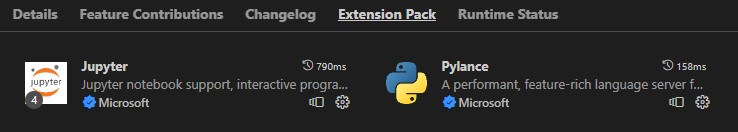
\includegraphics[scale=0.7]{Prt sc/Figure_9.jpg}
        \end{center}
    \end{figure}

    Однак \href{https://marketplace.visualstudio.com/items?itemName=ms-python.vscode-pylance}{\underline{Pylance}} є необов'язковий, 
    тобто розширення Python залишатиметься повністю функціональним без нього. Також є можливість його видалити без втрати функціоналу.

    \subsubsection{Налаштування середовища Python}
    \begin{enumerate}
        \item Виберіть інтерпретатор Python.
        \begin{figure}[h!]
            \begin{center}
                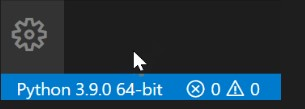
\includegraphics[scale=0.7]{Prt sc/Figure_10.jpg}
            \end{center}
        \end{figure}
\newpage
        \item Налаштуйте debugger через Debug Activity Bar.
        \begin{figure}[h!]
            \begin{center}
                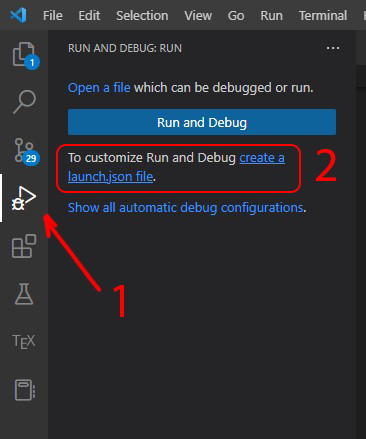
\includegraphics[scale=0.7]{Prt sc/Figure_11.jpg}
            \end{center}
        \end{figure}
        \item Обираємо поле "Flask" та натискаємо "Enter".
        \begin{figure}[h!]
            \begin{center}
                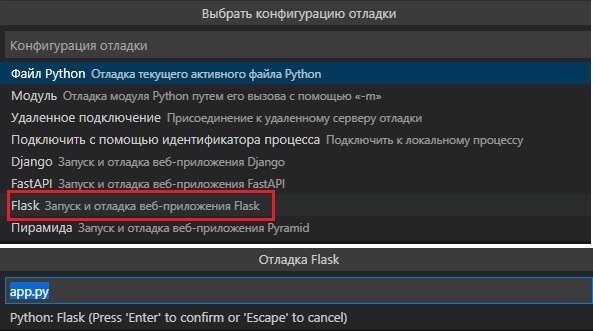
\includegraphics[scale=0.7]{Prt sc/Figure_12.jpg}
            \end{center}
        \end{figure}
\newpage
        \item У цьому файлі можна налаштувати середовище Python та усі встановлені плагіни.
        \begin{figure}[h!]
            \begin{center}
                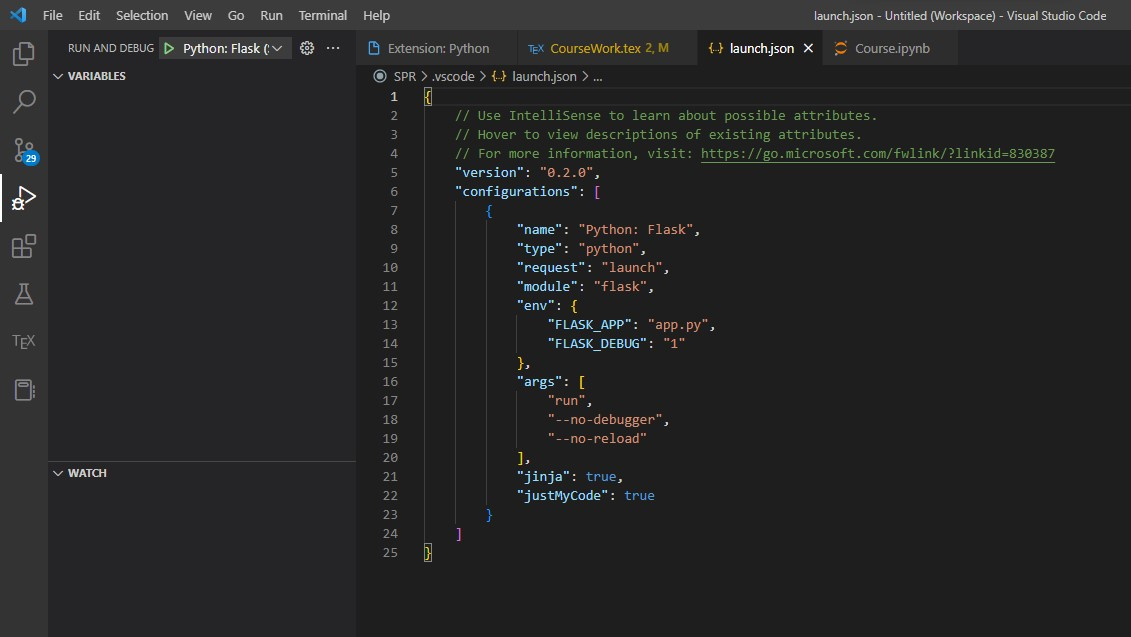
\includegraphics[scale=0.6]{Prt sc/Figure_13.jpg}
            \end{center}
        \end{figure}
    \end{enumerate}

\newpage
    \subsection {Початок роботи.}
    \hrulefill 
    \begin{figure}[h!]
        \begin{center}
            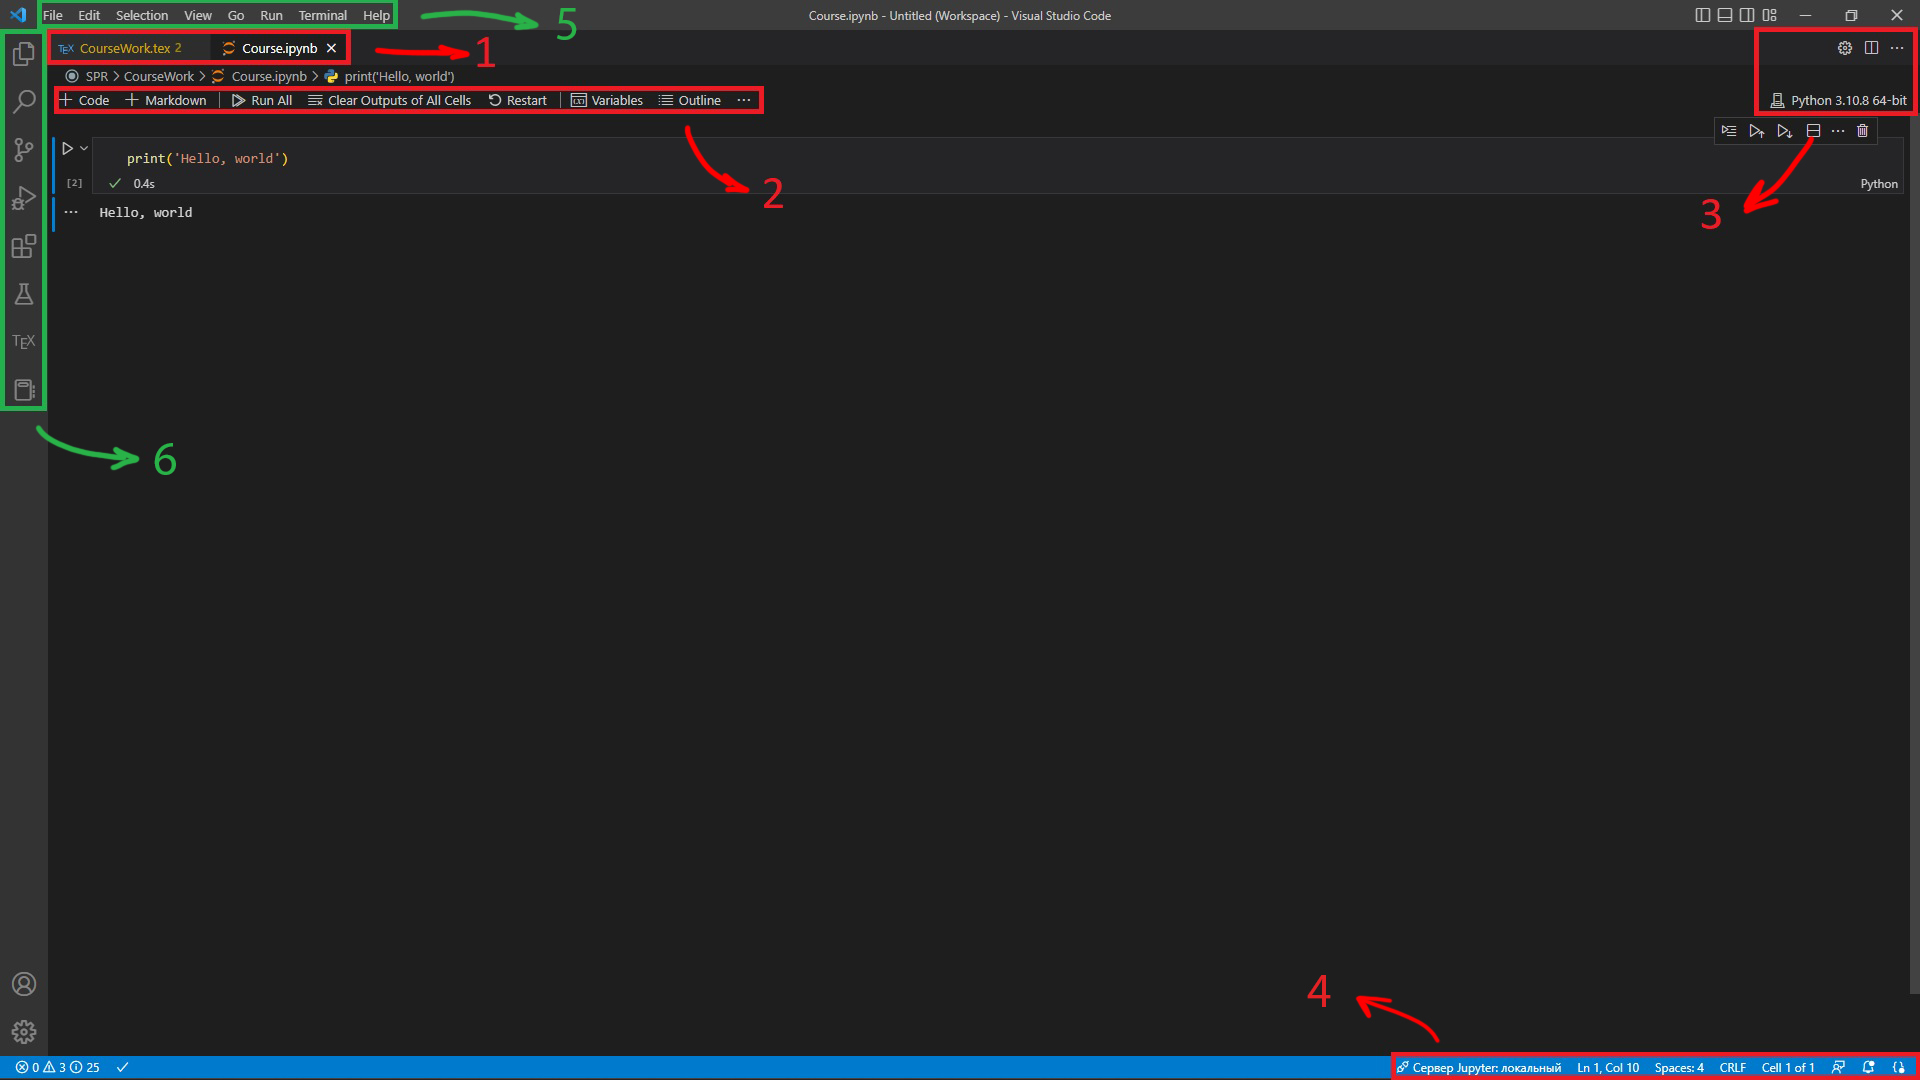
\includegraphics[scale=0.35]{Prt sc/Figure_6.jpg}
        \end{center}
    \end{figure}
    \begin{enumerate}
        \item Відкриті вкладки. Так званий Split editors.
        \item Панель взаємодії з Notebook.
        \begin{enumerate}
            \item[-] Створення комірки.
            \item[-] Додати markdown текст.
            \item[-] Виконати всі комірки.
            \item[-] Прибрати відображення вихідних даних в усіх комірках.
            \item[-] Перезавантажити комірки. 
            \item[-] Відкрити провідник змінних Jupyter Variables.
            \item[-] VS Code explorer.
        \end{enumerate}
        \item Панель налаштування середовища.
        \begin{enumerate}
            \item[-] Кастомізація Notebook, додавання нумерації, зміна теми, тощо...
            \item[-] Зміна ядра. Є можливість підключитися до Jupyter Server.
        \end{enumerate}
        \item Status bar.
        \item[5-6] Взаємодія з VS Code.
        \begin{enumerate}
            \item[-] Зберегти файл, створити, редагувати, переглянути, виконати, відкрити термінал, тощо...
            \item[-] VS Code explorer, пошук файлів, контроль версій (Git), дебаггер, "магазин" плагінів, встановлені плагіни.
        \end{enumerate}
    \end{enumerate}
\newpage
    \subsection {Source control(Git)}
    \hrulefill \\

    Source control - це клас систем, відповідальних за керування змінами в комп’ютерних програмах, документах, великих веб-сайтах чи інших колекціях інформації. 

    GitHub - це система для керування та контролю версіями за допомогою Git.

    Тобто за рахунок Git розробник може контролювати етапи створення свого проекту і в будь-який момент встановити попередню версію.
    \begin{center}
        \textbf{Етапи завантаження свого проект на платформу GitHub (за умови, що ви вже зареєстровані):}
    \end{center}
    \begin{enumerate}
        \item Натиснути комбінацію клавіш "Ctrl+Shift+G".
        \item Обираємо "Publish to GitHub".
        \item Оберіть папку, яку потріно експортувати.
        \item Авторизуйтесь зі свого аккаунту.
        \item Оберіть тип папки. Private - можете переглядати тільки власник. Public - відкрита для всіх на переглядат.
    \end{enumerate}
    \begin{figure}[h!]
        \begin{center}
            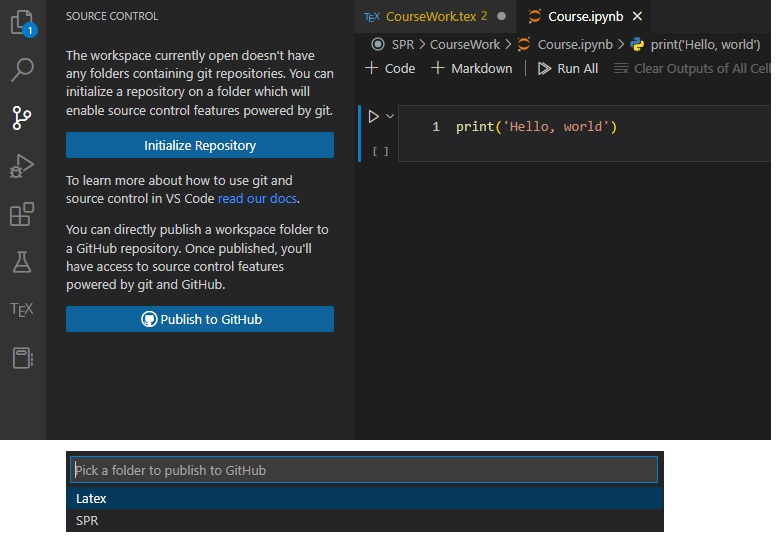
\includegraphics[scale=0.8]{Prt sc/Figure_7.jpg}
        \end{center}
    \end{figure}
\newpage
    Тепер усі зміни у проекті буду зберігатись на GitHub.
    \begin{figure}[h!]
        \begin{center}
            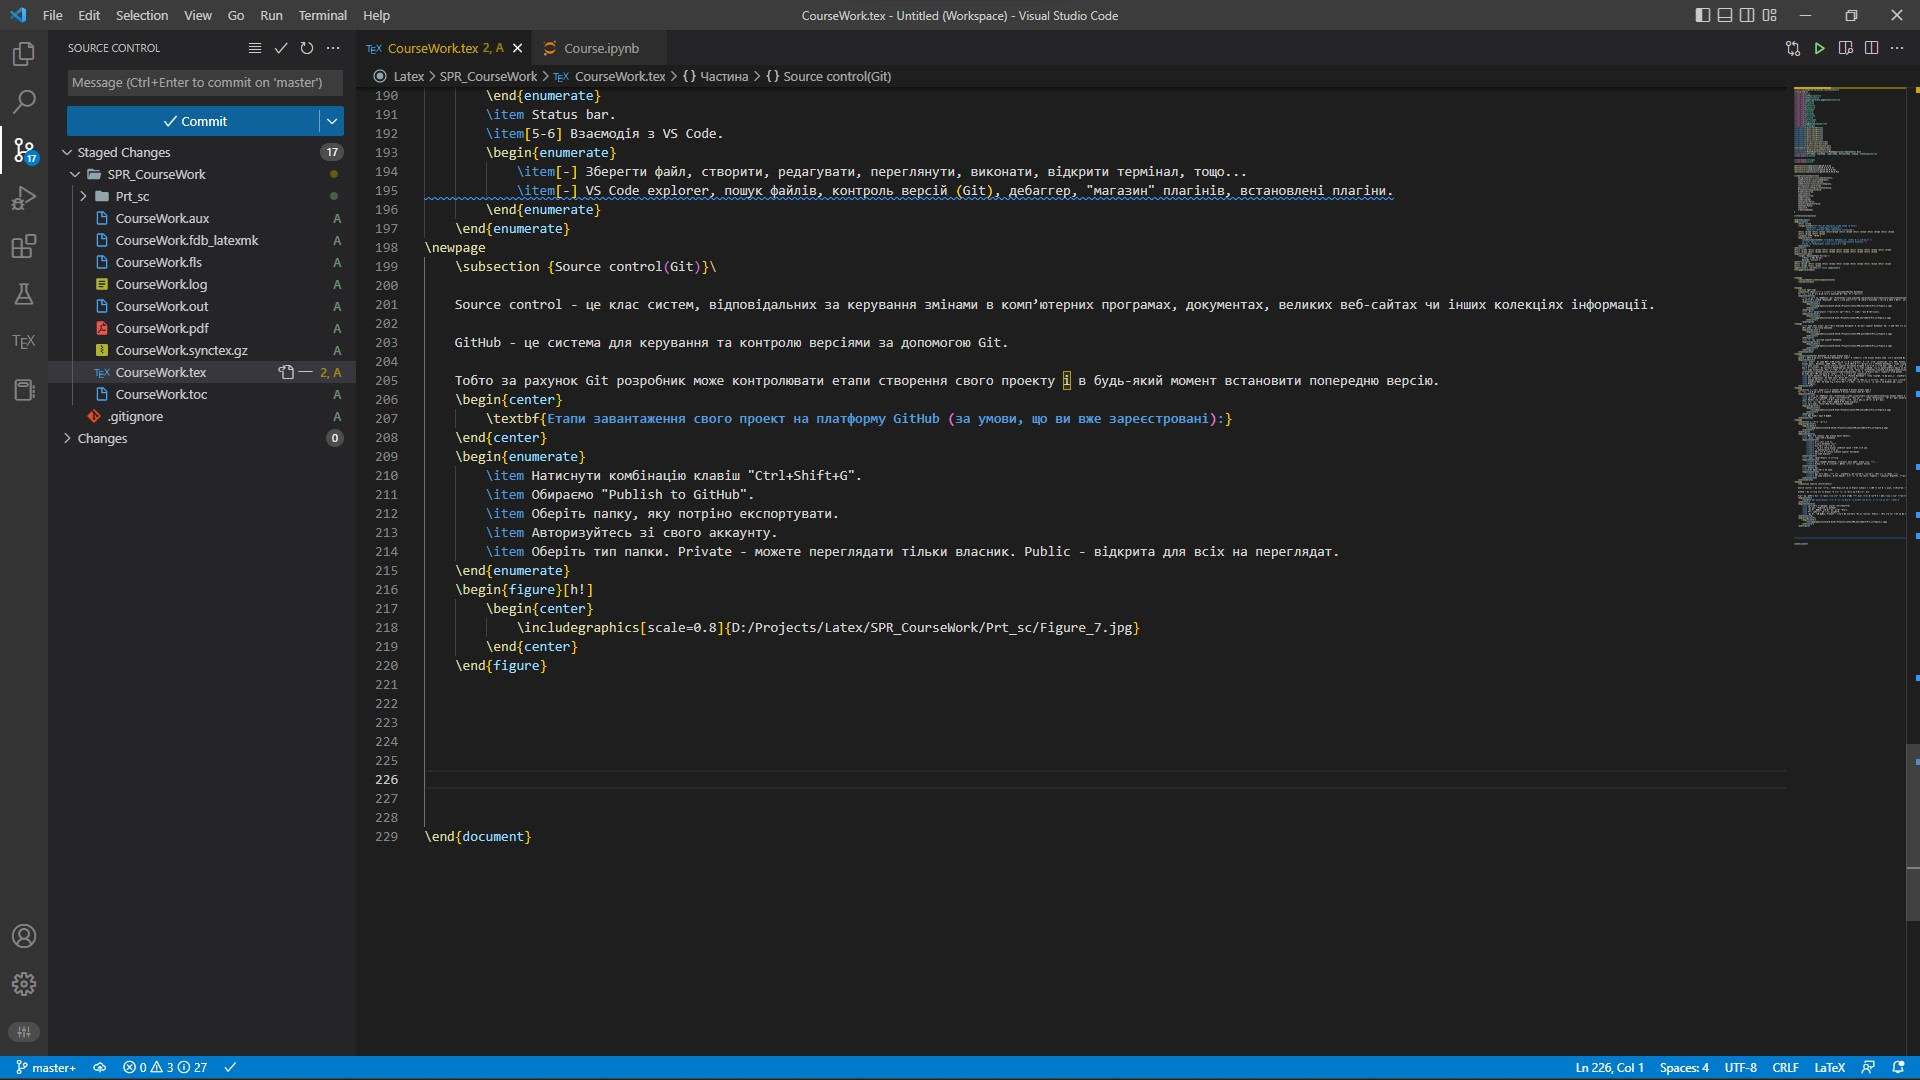
\includegraphics[scale=0.35]{Prt sc/Figure_8.jpg}
        \end{center}
    \end{figure}





\newpage
    \section{Частина}
    \subsection {Знайомство з датасетом.}
    \hrulefill \\
    Встановити \href{https://www.kaggle.com/datasets/thedevastator/get-your-game-on-metacritic-recommendations-and}{Cryptocurrency Prices Dataset} можна з сайту 
    \href{https://www.kaggle.com/}{Kaggle}.
    \begin{center}
        \textbf{About Dataset}
    \end{center}
    Цей набір даних містить історичні ціни та обсяги 4 криптовалют з 9 листопада 2017 року по 27 серпня 2022 року.
    \begin{itemize}
        \item BTC - Bitcoin
        \item BNB - Binance coin
        \item ETH - Ethereum
        \item USDT - Tether
    \end{itemize}
    \begin{figure}[h!]
        \begin{center}
            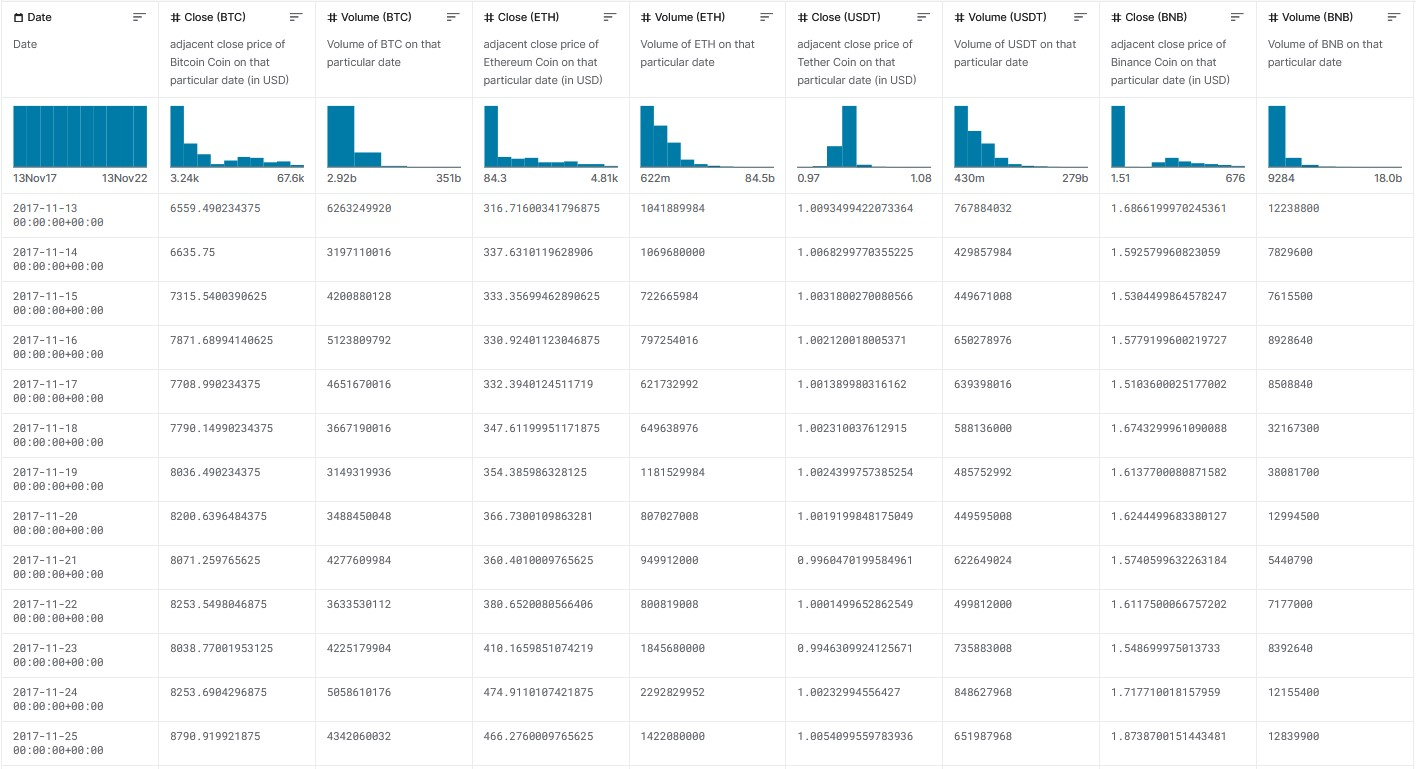
\includegraphics[scale=0.5]{Prt sc/Figure_14.jpg}
        \end{center}
    \end{figure}

    \subsection {Робота у середовищі IPython Notebook на модельних наборах даних.}
    \hrulefill \\
    
\end{document} 